\subsubsection{Tree-PM}

宇宙論$N$体シミュレーションの1スナップショットの加速度を計算する. FDPS
で作ったコードとGreeMを比較する. PMパートはGreeMから借用した. FFTは
fftw-3.3.4を使った.

{\bf 条件設定}

$N=32^3$の粒子を$\bm{0} \le \bm{x} < \bm{1}$の箱にランダムに分布させる.
$\theta=0.5$ (比較のために$\theta=0.0$も), $N_{\rm leaf}=10$, $N_{\rm
crit}=300$. $\Omega_0=0.3$. $\epsilon=2.5 \times 10^{-4}$. メッシュ長
$1/16(=2/N^{1/3})$. カットオフ半径$3/16$. プロセス数$2 \times 2 \times
2$. 各プロセスで粒子配列の順番がFDPSとGreeMで全く同じになるようにした.

{\bf 結果}

PM forceはGreeMとFDPSで完全に一致した.

図\ref{fig:comparison_pp}はPP forceの結果($\theta=0.0$). GreeMとFDPSの
相対誤差の最大は$0.1$\%を越えるくらい. これは, Phantom-GRAPEの誤差によ
るもの. Tanikawa et al. (2012, NewA, 19, 74)のfig.~8を見るとわかるが,
力が最も大きいところで最も相対誤差が大きく$0.1$\%程度 (ここで使っている
$E$と$F$はこの論文のものと同じ).

図\ref{fig:comparison_pt05}はツリーの検証. GreeMとFDPSの$\theta=0.5$の相
対誤差分布はほぼ同じ. GreeMとFDPSの$\theta=0.5$同士の差の方が小さい.

図\ref{fig:comparison_pt10}はツリーの検証. GreeMとFDPSの$\theta=1.0$の相
対誤差分布はほぼ同じ. GreeMとFDPSの$\theta=1.0$同士の差の方が小さい.

\begin{figure}
  \begin{center}
    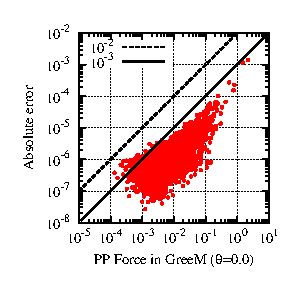
\includegraphics[width=10cm,bb=0 0 170 170]{fig/comparison_pp.eps}
  \end{center}
  \caption{GreeMのPP forceの絶対値(横軸)と, GreeMとFDPSのPP forceの絶対
    誤差(縦軸). ツリーの精度は$\theta=0.0$.}
  \label{fig:comparison_pp}
\end{figure}

\begin{figure}
  \begin{center}
    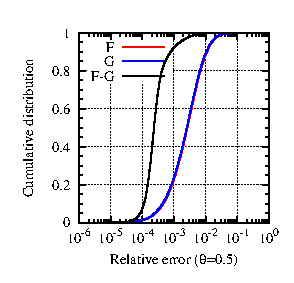
\includegraphics[width=10cm,bb=0 0 170 170]{fig/comparison_pt05.eps}
  \end{center}
  \caption{(赤)FDPSのPP forceの相対誤差($\theta=0.0$と$0.5$を比較).
    (青)GreeMのPP forceの相対誤差($\theta=0.0$と$0.5$を比較). (黒)FDPS
    とGreeMのPP forceの相対誤差(どちらも$\theta=0.5$).}
  \label{fig:comparison_pt05}
\end{figure}

\begin{figure}
  \begin{center}
    \includegraphics[width=10cm,bb=0 0 170 170]{fig/comparison_pt10.eps}
  \end{center}
  \caption{(赤)FDPSのPP forceの相対誤差($\theta=0.0$と$1.0$を比較).
    (青)GreeMのPP forceの相対誤差($\theta=0.0$と$1.0$を比較). (黒)FDPS
    とGreeMのPP forceの相対誤差(どちらも$\theta=1.0$).}
  \label{fig:comparison_pt10}
\end{figure}
